\subsection{Paquete 5: Gestión financiera compartida}

    El paquete resuelve la contabilidad compartida entre compañeros de piso. Registra facturas con repartos proporcionales, simplifica grafos de deuda para minimizar transferencias cruzadas y almacena recibos de liquidación directa. La figura \ref{fig:dcu_gastos} detalla las relaciones con los siete casos de uso financieros (CU50 a CU56).

\begin{figure}[H]
    \centering
    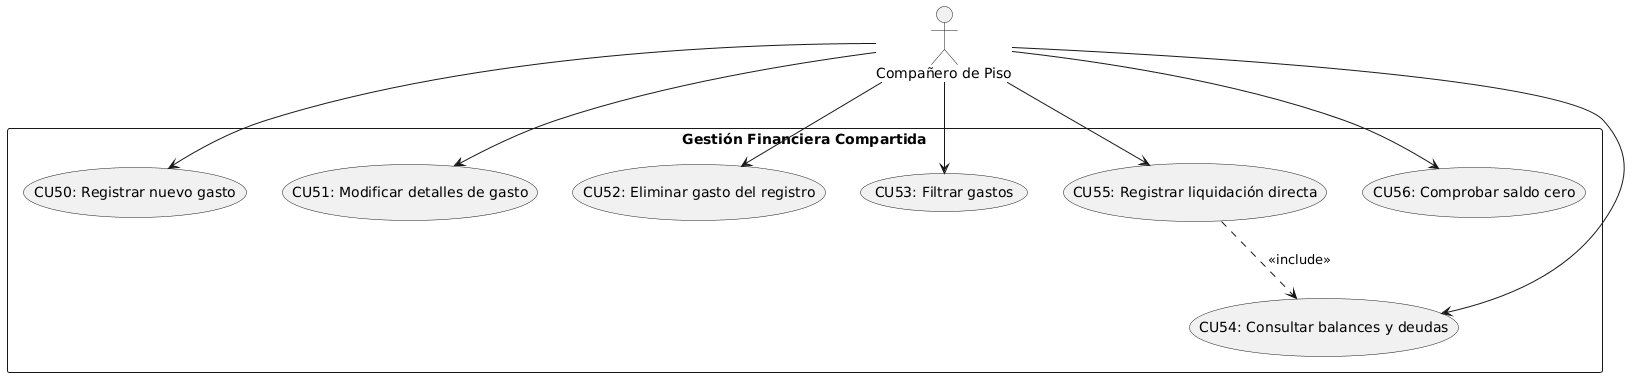
\includegraphics[width=0.75\textwidth]{AnalisisFuncional/img/dcu_gastos.png}
    \caption{Diagrama de casos de uso de gestión financiera compartida}
    \label{fig:dcu_gastos}
\end{figure}

    Las fichas tabulares desglosan los casos de uso CU50 a CU56:

\begin{table}[H]
\centering
\begin{tabular}{|p{3.2cm}|p{11.3cm}|}
\hline
\textbf{Caso de Uso} & \textbf{CU50: Registrar nuevo gasto con reparto} \\ \hline
\textbf{Actores} & Compañero de Piso \\ \hline
\textbf{Descripción} & Introduce un gasto abonado por un miembro distribuyendo el coste entre los integrantes \\ \hline
\textbf{Precondiciones} & Ser miembro activo del hogar con al menos otro compañero vinculado \\ \hline
\textbf{Flujo básico} & 
1. El compañero accede al formulario de gastos e introduce importe, concepto y fecha. \newline
2. El compañero selecciona los participantes asignados al reparto de la cuota. \newline
3. El sistema valida la consistencia matemática entre el total y los importes desglosados. \newline
4. El backend registra la transacción contable y actualiza de inmediato los saldos consolidados. \\ \hline
\end{tabular}
\caption{Especificación del caso de uso CU50}
\label{tab:cu50}
\end{table}

\begin{table}[H]
\centering
\begin{tabular}{|p{3.2cm}|p{11.3cm}|}
\hline
\textbf{Caso de Uso} & \textbf{CU51: Modificar detalles o reparto de gasto} \\ \hline
\textbf{Actores} & Compañero de Piso \\ \hline
\textbf{Descripción} & Permite actualizar la cuantía, concepto o miembros implicados en un gasto registrado \\ \hline
\textbf{Precondiciones} & Ser el creador del registro del gasto y que no pertenezca a un período cerrado \\ \hline
\textbf{Flujo básico} & 
1. El compañero localiza el asiento contable y pulsa sobre la opción de edición. \newline
2. El compañero corrige el importe o reconfigura los miembros que participan. \newline
3. El sistema recalcula las diferencias deudoras y acreedoras asociadas. \newline
4. El backend actualiza la entidad persistida y ajusta los balances generales del hogar. \\ \hline
\end{tabular}
\caption{Especificación del caso de uso CU51}
\label{tab:cu51}
\end{table}

\begin{table}[H]
\centering
\begin{tabular}{|p{3.2cm}|p{11.3cm}|}
\hline
\textbf{Caso de Uso} & \textbf{CU52: Eliminar gasto del registro} \\ \hline
\textbf{Actores} & Compañero de Piso \\ \hline
\textbf{Descripción} & Suprime un gasto registrado previamente revirtiendo su impacto en los balances \\ \hline
\textbf{Precondiciones} & Ostentar la autoría del apunte contable \\ \hline
\textbf{Flujo básico} & 
1. El compañero selecciona el gasto y solicita su retirada formal del historial. \newline
2. El sistema pide confirmación explícita indicando el ajuste contable consecuente. \newline
3. El backend anula la imputación de deuda y restituye los saldos previos de cada miembro. \newline
4. El sistema notifica la supresión del registro en el panel de actividad del piso. \\ \hline
\end{tabular}
\caption{Especificación del caso de uso CU52}
\label{tab:cu52}
\end{table}

\begin{table}[H]
\centering
\begin{tabular}{|p{3.2cm}|p{11.3cm}|}
\hline
\textbf{Caso de Uso} & \textbf{CU53: Filtrar gastos por fechas y participantes} \\ \hline
\textbf{Actores} & Compañero de Piso \\ \hline
\textbf{Descripción} & Permite segmentar el histórico de gastos según intervalos de tiempo o miembros \\ \hline
\textbf{Precondiciones} & Pertenecer al espacio de convivencia consultado \\ \hline
\textbf{Flujo básico} & 
1. El usuario accede a la pestaña de histórico contable en el panel de gastos. \newline
2. El usuario define un rango de fechas, un pagador concreto o un estado de liquidación. \newline
3. El sistema consulta las transacciones coincidentes y devuelve la lista paginada. \newline
4. La interfaz recalcula y muestra la suma total de las operaciones filtradas. \\ \hline
\end{tabular}
\caption{Especificación del caso de uso CU53}
\label{tab:cu53}
\end{table}

\begin{table}[H]
\centering
\begin{tabular}{|p{3.2cm}|p{11.3cm}|}
\hline
\textbf{Caso de Uso} & \textbf{CU54: Consultar balances y transferencias sugeridas} \\ \hline
\textbf{Actores} & Compañero de Piso \\ \hline
\textbf{Descripción} & Muestra el estado neto de saldos y la propuesta óptima de pagos para saldar deudas \\ \hline
\textbf{Precondiciones} & Estar formalmente integrado en el hogar \\ \hline
\textbf{Flujo básico} & 
1. El compañero entra en la vista de balances compartidos. \newline
2. El sistema procesa la matriz de deudas aplicando el algoritmo de simplificación de transferencias. \newline
3. La interfaz visualiza a quién debe dinero cada miembro o cuánto debe percibir. \newline
4. El sistema expone las transacciones sugeridas con importes mínimos para saldar cuentas. \\ \hline
\end{tabular}
\caption{Especificación del caso de uso CU54}
\label{tab:cu54}
\end{table}

\begin{table}[H]
\centering
\begin{tabular}{|p{3.2cm}|p{11.3cm}|}
\hline
\textbf{Caso de Uso} & \textbf{CU55: Registrar liquidación directa} \\ \hline
\textbf{Actores} & Compañero de Piso \\ \hline
\textbf{Descripción} & Asienta un pago directo efectuado entre dos compañeros para compensar una deuda \\ \hline
\textbf{Precondiciones} & Mantener un saldo deudor pendiente respecto al destinatario de la compensación \\ \hline
\textbf{Flujo básico} & 
1. El deudor accede a la lista de transferencias sugeridas y pulsa liquidar saldo. \newline
2. Se invoca de forma obligatoria la consulta de balances y transferencias sugeridas. \newline
3. El usuario confirma el importe transferido y el método de pago utilizado. \newline
4. El backend asienta la liquidación y actualiza los saldos de ambos compañeros a cero. \\ \hline
\end{tabular}
\caption{Especificación del caso de uso CU55}
\label{tab:cu55}
\end{table}

\begin{table}[H]
\centering
\begin{tabular}{|p{3.2cm}|p{11.3cm}|}
\hline
\textbf{Caso de Uso} & \textbf{CU56: Comprobar saldo cero} \\ \hline
\textbf{Actores} & Compañero de Piso \\ \hline
\textbf{Descripción} & Valida automáticamente que un miembro no posea deudas activas ni acreencias en el piso \\ \hline
\textbf{Precondiciones} & Estar en proceso de abandono o expulsión del espacio de convivencia \\ \hline
\textbf{Flujo básico} & 
1. El sistema intercepta una solicitud de baja voluntaria o expulsión de un miembro. \newline
2. El backend computa el balance neto acumulado del usuario en todos los gastos registrados. \newline
3. Si el saldo es exactamente cero, el sistema confirma la validación favorablemente. \newline
4. Si existe balance positivo o negativo, el sistema bloquea la operación e indica la liquidación previa. \\ \hline
\end{tabular}
\caption{Especificación del caso de uso CU56}
\label{tab:cu56}
\end{table}